\documentclass[11pt]{charter}
% !TeX spellcheck = es
% El títulos de la memoria, se usa en la carátula y se puede usar el cualquier lugar del documento con el comando \ttitle
\titulo{Sistema de actualización remota de firmware a través de una red LoRaWAN} 

% Nombre del posgrado, se usa en la carátula y se puede usar el cualquier lugar del documento con el comando \degreename
\posgrado{Carrera de Especialización en Sistemas Embebidos} 
%\posgrado{Carrera de Especialización en Internet de las Cosas} 
%\posgrado{Carrera de Especialización en Intelegencia Artificial}
%\posgrado{Maestría en Sistemas Embebidos} 
%\posgrado{Maestría en Internet de las cosas}

% Tu nombre, se puede usar el cualquier lugar del documento con el comando \authorname
\autor{Ronal Celaya} 

% El nombre del director y co-director, se puede usar el cualquier lugar del documento con el comando \supname y \cosupname y \pertesupname y \pertecosupname
\director{Nombre del Director}
\pertenenciaDirector{pertenencia} 
% FIXME:NO IMPLEMENTADO EL CODIRECTOR ni su pertenencia
\codirector{} % si queda vacio no se deberíá incluir 
\pertenenciaCoDirector{}

% Nombre del cliente, quien va a aprobar los resultados del proyecto, se puede usar con el comando \clientename y \empclientename
\cliente{Osvaldo Ivani}
\empresaCliente{SMARTIUM, S. A.}

% Nombre y pertenencia de los jurados, se pueden usar el cualquier lugar del documento con el comando \jurunoname, \jurdosname y \jurtresname y \perteunoname, \pertedosname y \pertetresname.
\juradoUno{Nombre y Apellido (1)}
\pertenenciaJurUno{pertenencia (1)} 
\juradoDos{Nombre y Apellido (2)}
\pertenenciaJurDos{pertenencia (2)}
\juradoTres{Nombre y Apellido (3)}
\pertenenciaJurTres{pertenencia (3)}
 
\fechaINICIO{27 de junio de 2020}		%Fecha de inicio de la cursada de GdP \fechaInicioName
\fechaFINALPlanificacion{22 de Agosto de 2020} 	%Fecha de final de cursada de GdP
\fechaFINALTrabajo{22 de diciembre de 2020}		%Fecha de defensa pública del trabajo final


\begin{document}

\maketitle
\thispagestyle{empty}
\pagebreak


\thispagestyle{empty}
{\setlength{\parskip}{0pt}
\tableofcontents{}
}
\pagebreak


\section{Registros de cambios}
\label{sec:registro}


\begin{table}[ht]
\label{tab:registro}
\centering

\begin{tabularx}{\linewidth}{@{}|c|X|c|@{}}
\hline
\rowcolor[HTML]{C0C0C0} 
Revisión & \multicolumn{1}{c|}{\cellcolor[HTML]{C0C0C0}Detalles de los cambios realizados} & Fecha      \\ \hline
1.0      & Creación del documento                                                          & 27/06/2020 \\ \hline
1.1      & Desarrollo de las secciones 1 hasta la 6										   & 09/07/2020 \\ \hline
\end{tabularx}
\end{table}

\pagebreak



\section{Acta de Constitución del Proyecto}
\label{sec:acta}

\begin{flushright}
Buenos Aires, \fechaInicioName
\end{flushright}

\vspace{2cm}

Por medio de la presente se acuerda con el Ing. \authorname\hspace{1px} que su Trabajo Final de la \degreename\hspace{1px} se titulará ``\ttitle'', consistirá esencialmente en el prototipo preliminar de un \textcolor{black}{sistema que realice la actualización remota de firmware (FUOTA, por sus siglas en inglés Firmware Update Over The Air) a través de una red LoRaWAN.}, y tendrá un presupuesto preliminar estimado de 600 hs de trabajo, con fecha de inicio \fechaInicioName\hspace{1px} y fecha de presentación pública \fechaFinalName.

Se adjunta a esta acta la planificación inicial.

\vfill

% Esta parte se construye sola con la información que hayan cargado en el preámbulo del documento y no debe modificarla
\begin{table}[ht]
\centering
\begin{tabular}{ccc}
\begin{tabular}[c]{@{}c@{}}Ariel Lutenberg \\ Director posgrado FIUBA\end{tabular} &  & \begin{tabular}[c]{@{}c@{}}\clientename \\ \empclientename \end{tabular} \vspace{2.5cm} \\ 
\multicolumn{3}{c}{\begin{tabular}[c]{@{}c@{}} \supname \\ Director del Trabajo Final\end{tabular}} \vspace{2.5cm} \\
\begin{tabular}[c]{@{}c@{}}\jurunoname \\ Jurado del Trabajo Final\end{tabular}     &  & \begin{tabular}[c]{@{}c@{}}\jurdosname\\ Jurado del Trabajo Final\end{tabular}  \vspace{2.5cm}  \\
\multicolumn{3}{c}{\begin{tabular}[c]{@{}c@{}} \jurtresname\\ Jurado del Trabajo Final\end{tabular}} \vspace{.5cm}                                                                     
\end{tabular}
\end{table}




\section{Descripción técnica-conceptual del Proyecto a realizar}
\label{sec:descripcion}

\begin{consigna}{black}
El sector del IoT o internet de las cosas, tiene previsto un crecimiento a una tasa cercana
al 10% anual durante los próximos 10 años según varias fuentes reconocidas.
Actualmente, en el 2020, la cuota de este mercado ronda los 900 mil millones de dólares
estadounidenses, y se prevé que sobrepase los 2 billones para el 2028. Una de las
características de este tipo de redes es la mantenibilidad, en donde, si se realizara un
despliegue de miles de dispositivos y se tuviera que realizar una inclusión de
funcionalidad o solución de alguna vulnerabilidad, es de crucial importancia poder hacerlo
sin realizar una recogida de los dispositivos desplegados y reprogramarlos manualmente.
En el ámbito del agro argentino muchas veces los dispositivos son instalados en zonas
remotas, en las que ir a buscarlos se traduce en altos costos y tiempo invertido por la
empresa.

El sistema embebido a desarrollar debe permitir la actualización remota del firmware de
un microcontrolador de la serie STM32L151 a través de una sesión multicast de
LoRaWAN. Para esto se debe diseñar un sistema que cumpla con las especificaciones de
sesiones multicast, de fragmentación y actualización remota establecidas por la LoRa
Alliance\textregistered. El sistema debe contar con un algoritmo capaz de permitir la reprogramación de la memoria interna del microcontrolador desde una memoria externa del tipo que
corresponda.

La transmisión y recepción de toda la información que se requiera, se deberá realizar a
través de una red LoRaWAN usando la banda AU915 y la versión del protocolo 1.0.2
revisión B. El hardware adicional que se utilice en el desarrollo debe estar orientado a
opciones de bajo consumo, y debe estar optimizado por software para maximizar el
rendimiento del procesamiento y la comunicación. El algoritmo que se implemente debe
ser tolerante a fallas y debe validar la integridad y autenticidad del firmware que reciba.

En la Figura \ref{fig:diagBloquesNivel1} se observa el digrama de bloques funcionales del sistema. En esta, se destacan cuatro bloques principales: Transceptor LoRa, Flash externa, Microcontrolador y LED de indicación de estado. Cada bloque presenta diferentes retos de diseño.

El Transceptor LoRa se encargará de recibir las tramas segmentadas del firmware para luego ensamblarlas y guardarlas en la Flash externa. El Microcontrolador es parte del sistema ya existente; este debe ser estudiado para considerar la actualización del bootloader y adecuarlo a la nueva funcionalidad. En el diagrama no se consideran los elementos para alimentación del sistema.

\vspace{25px}

\begin{figure}[htpb]
\centering 
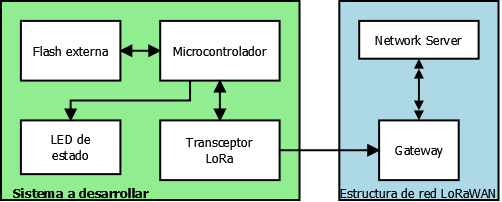
\includegraphics[width=.7\textwidth]{./Figuras/diagramaDeBloquesNivel1.png}
\caption{Diagrama en bloques del sistema}
\label{fig:diagBloquesNivel1}
\end{figure}

\vspace{25px}

Al entrar en el detalle del Transceptor LoRa, en la Figura \ref{fig:diagBloquesNivel2} se puede observar mejor los componentes del sistema. Existen tres partes importantes tanto del lado del servidor como del cliente. Estos bloques los define la recomendación técnica de la LoRa Alliance\textregistered. Los tres bloques son: Multicast usado para generar una ventana para la transmisión, Fragmentación que se encarga de fragmentar los paquetes a enviar y Sincornización de Relojes cuyo trabajo es asegurar la sincronización del dispositivo a actualizar con el sistema. Al rededor de ellos coexisten el Servidor de Actualización de Firmware que es el encargado de generar el firmware para la actualización. Tanto el servidor como el cliente están enlazados a través de un link LoRaWAN.

\vspace{25px}

\begin{figure}[htpb]
\centering 
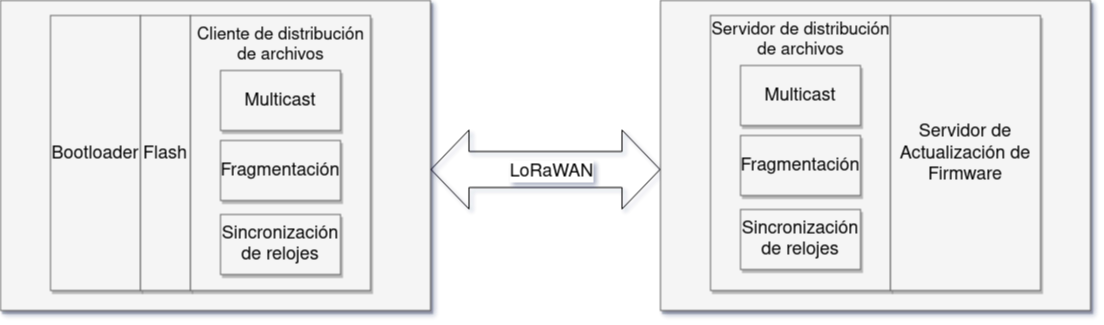
\includegraphics[width=.9\textwidth]{./Figuras/diagramaDeBloquesNivel2.png}
\caption{Diagrama en bloques del sistema}
\label{fig:diagBloquesNivel2}
\end{figure}

\vspace{25px}


\end{consigna}


\section{Identificación y análisis de los interesados}
\label{sec:interesados}
A continuación se presentan los interesados involucrados en el desarrollo del proyecto.
\begin{consigna}{black} 
\begin{table}[ht]
%\caption{Identificación de los interesados}
%\label{tab:interesados}
\begin{tabularx}{\linewidth}{@{}|l|X|X|l|@{}}
\hline
\rowcolor[HTML]{C0C0C0} 
Rol           & Nombre y Apellido & Organización 	& Puesto 	\\ \hline
Cliente       & \clientename      &\empclientename	& Gerente de Ingeniería       	\\ \hline
Responsable   & \authorname       & FIUBA        	& Alumno 	\\ \hline
Colaboradores & Jhonattan Camargo &\empclientename  &Ingeniería de desarrollo \\ \hline
Orientador    & \supname	      & \pertesupname 	& Director	Trabajo final \\ \hline
Usuario final & Personal técnico o capacitado                  &              	&        	\\ \hline
\end{tabularx}
\end{table}

\begin{itemize}
\item Cliente: \clientename, Gerente de Ingeniería y el encargado del proyecto por parte de la empresa.
\item Colaborador: Jhonattan Camargo, Ingeniero en la empresa. Conocimiento técnico del proyecto y contacto directo ante cualquier duda.
\end{itemize}

\end{consigna}

\section{1. Propósito del proyecto}
\label{sec:proposito}

\begin{consigna}{black}
El proposito del proyecto es lograr un sistema que realice la actualización remota de firmware (FUOTA, por
sus siglas en inglés Firmware Update Over The Air) a través de una red LoRaWAN. El
dispositivo debe ser capaz de realizar la actualización a través de una memoria flash
externa en la que se guardarán las tramas recibidas inalambricamente.
\end{consigna}

\section{2. Alcance del proyecto}
\label{sec:alcance}

\begin{consigna}{black}
El presente proyecto incluira:
\begin{itemize}
	\item Diseño de PCB del prototipo.
	\item Desarrollo de bootloader.
	\item Desarrollo de algoritmos para firma y verificación de firmware.
	\item Desarrollo de la fase de negociación de la ventana de distribución.
	\item Desarrollo de la fase fragmentación y ensamblaje de los paquetes a transmitir.
	\item Desarrollo de la fase de sincronización de relojes.
\end{itemize}

El presente proyecto no incluirá:
\begin{itemize}
	\item Desarrollo del servidor de red.
	\item Desarrollo del hardware a actualizar.
	\item Desarrollo de firmwares específicos.
	\item Desarrollo del gateway.
\end{itemize}

\end{consigna}


\section{3. Supuestos del proyecto}
\label{sec:supuestos}

\begin{consigna}{black}
Para el desarrollo del presente proyecto se supone que se cuenta con lo siguiente:

\begin{itemize}
\item Kits de desarrollo para LoraWAN.
\item Hardware funcional que se usará para pruebas de actualización.
\item Gateway Lora.
\item Servidor donde correrán las aplicaciones.
\end{itemize}

La empresa también está comprometida a proveer espacios de trabajo si son necesarios.
\end{consigna}

\section{4. Requerimientos}
\label{sec:requerimientos}
\begin{consigna}{black}
Los requerimientos funcionales y no funcionales del proyecto son los siguientes:
\begin{enumerate}
\item Requerimientos funcionales.
	\begin{enumerate}
	\item El sistema debe ser capaz de actualizar el firmware de un dispositvo usando la red LoRaWAN.
	\item El usuario debe ser capaz de elegir que dispositivo quiere actualizar.
	\item El usuario debe poder seleccionar el firmware a ser actualizado.
	\item El sistema debe permitir al usuario leer la versión del firmware en el dispositivo a ser actualizado.
	\item El sistema debe proveer una manera para asegurar la integridad del firmware.
	\item El sistema debe proveer al usuario opciones de firmado del firmware.
	\item El usuario debe estar en la capacidad de seleccionar la cantidad de fragmentos que se usaran en la transmisión del firmware.
	\end{enumerate}
\item Requerimientos no funcionales.
	\begin{enumerate}
	\item Requerimientos del sistema.
	\begin{enumerate}
		\item El sistema debe basarse en las especificaciones establecidas por la LoRa Alliance\textregistered.
		\item El sistema debe usar una memoria externa para almacenar la actualización del firmware.
		\item La transmisión del firmware debe ser tolerante a fallas.
		\item El sistema usará dispositivos que aseguren el bajo consumo de energía.
		\item El software debe estar optimizado para lograr un equilibrio entre rendimiento y consumo de energía.
		\item El o los algoritmos usados deben asegurar la integridad y autenticidad del firmware a actualizar.
	\end{enumerate}
	\item Requerimientos de documentación
	\begin{itemize}
		\item Antes de comenzar el la implementación del proyecto debe existir un documento donde se contemple la planificación inicial.
		\item Se debe entregar una memoria donde se describa el diseño y funcionamiento del sistema.
	\end{itemize}
    \item Requerimientos de procesos
    \begin{itemize}
    	\item Se debe poder hacer una revisión del proyecto de manera semanal para poder hacer correcciones tempranas
    	\item Se usará un sistema de control de versión para el código y documentación del proyecto.
    \end{itemize}
	\end{enumerate}
\end{enumerate}

\end{consigna}

\section{5. Entregables principales del proyecto}
\label{sec:entregables}

\begin{consigna}{black}
Los entregables del proyecto serán:
\begin{itemize}
\item Memoria descriptiva del proyecto.
\item Prototipo para la actualización del firmware.
\item Manual de utilización.
\item Diagramas esquemáticos.
\item Código fuente.

\end{itemize}

\end{consigna}

\section{6. Desglose del trabajo en tareas}
\label{sec:wbs}

\begin{consigna}{black}
Para la realización de este proyecto se consideran las siguientes tareas:

\begin{enumerate}
	\item Planificación. \hfill(62 hs)
	\begin{enumerate}
		\item Estudio de las especificacione.s \hfill(4 hs)
		\item Realización del documento de planificación. \hfill(15 hs)
		\item Revisión de la planificación. \hfill(3 hs)
		\item Reuniones semanales. \hfill(32 hs)
		\item Reuniones mensuales. \hfill(8 hs)
	\end{enumerate}
	\item Documentación bibliográfica e Investigación. (75 hs)
	\begin{enumerate}
		\item Estudio del protocolo LoRa y LoRaWAN. \hfill(25 hs)
		\item Estudio de las especificaiones de FUOTA de la LoRa Alliance\textregistered. \hfill(20 hs)
		\item Estudio de las soluciones existentes. \hfill(20 hs)
		\item Estudio de las especificaciones del hardware. \hfill(10 hs)
	\end{enumerate}
	\item Desarrollo del software. \hfill(210 hs)
	\begin{enumerate}
		\item Diseño de arquitectura. \hfill(20 hs)
		\item Pruebas de comunicación iniciales. \hfill(10 hs)
		\item Implementación de la fase de firma y verificación del firmware. \hfill(40 hs)
		\item Implementación de la fase de negociación de banda para la transmisión. \hfill(40 hs)
		\item Implementación de la fase de fragmentación y ensamblaje del firmware. \hfill(40 hs)
		\item Implementación de la fase de sincronización de relojes. \hfill(40 hs)
		\item Integración de los módulos del sistema. \hfill(20 hs)
	\end{enumerate}
    \item Desarrollo de hardware. \hfill(115 hs)
    \begin{enumerate}
    	\item Seleción de elementos constitutivos del prototipo. \hfill(5 hs)
    	\item Diseño de la arquitectura. \hfill(10 hs)
    	\item Diseño del diagrama esquemático. \hfill(30 hs)
    	\item Diseño del PCB. \hfill(30 hs)
    	\item Ensamblaje del prototipo. \hfill(40 hs)
    \end{enumerate}
	\item Pruebas en Integración. \hfill(40 hs)
	\begin{enumerate}
		\item Pruebas de integración y funcionalidad. \hfill(40 hs)
	\end{enumerate}
	\item Documentación del proyecto. \hfill(100 hs)
	\begin{enumerate}
		\item Informe de de avance. \hfill(20 hs)
		\item Elaboración del manual del sistema. \hfill(20 hs)
		\item Memoria final del proyecto. \hfill(40 hs)
		\item Presentación final del proyecto. \hfill(20 hs)
	\end{enumerate}
    	
\end{enumerate}

Cantidad total de horas: (602 hs).

\end{consigna}

\section{7. Diagrama de Activity On Node}
\label{sec:AoN}

\begin{consigna}{red}
Armar el AoN a partir del WBS definido en la etapa anterior. 

%La figura \ref{fig:AoN} fue elaborada con el paquete latex tikz y pueden consultar la siguiente referencia \textit{online}:

%\url{https://www.overleaf.com/learn/latex/LaTeX_Graphics_using_TikZ:_A_Tutorial_for_Beginners_(Part_3)\%E2\%80\%94Creating_Flowcharts}

\end{consigna}

\begin{figure}[htpb]
\centering 
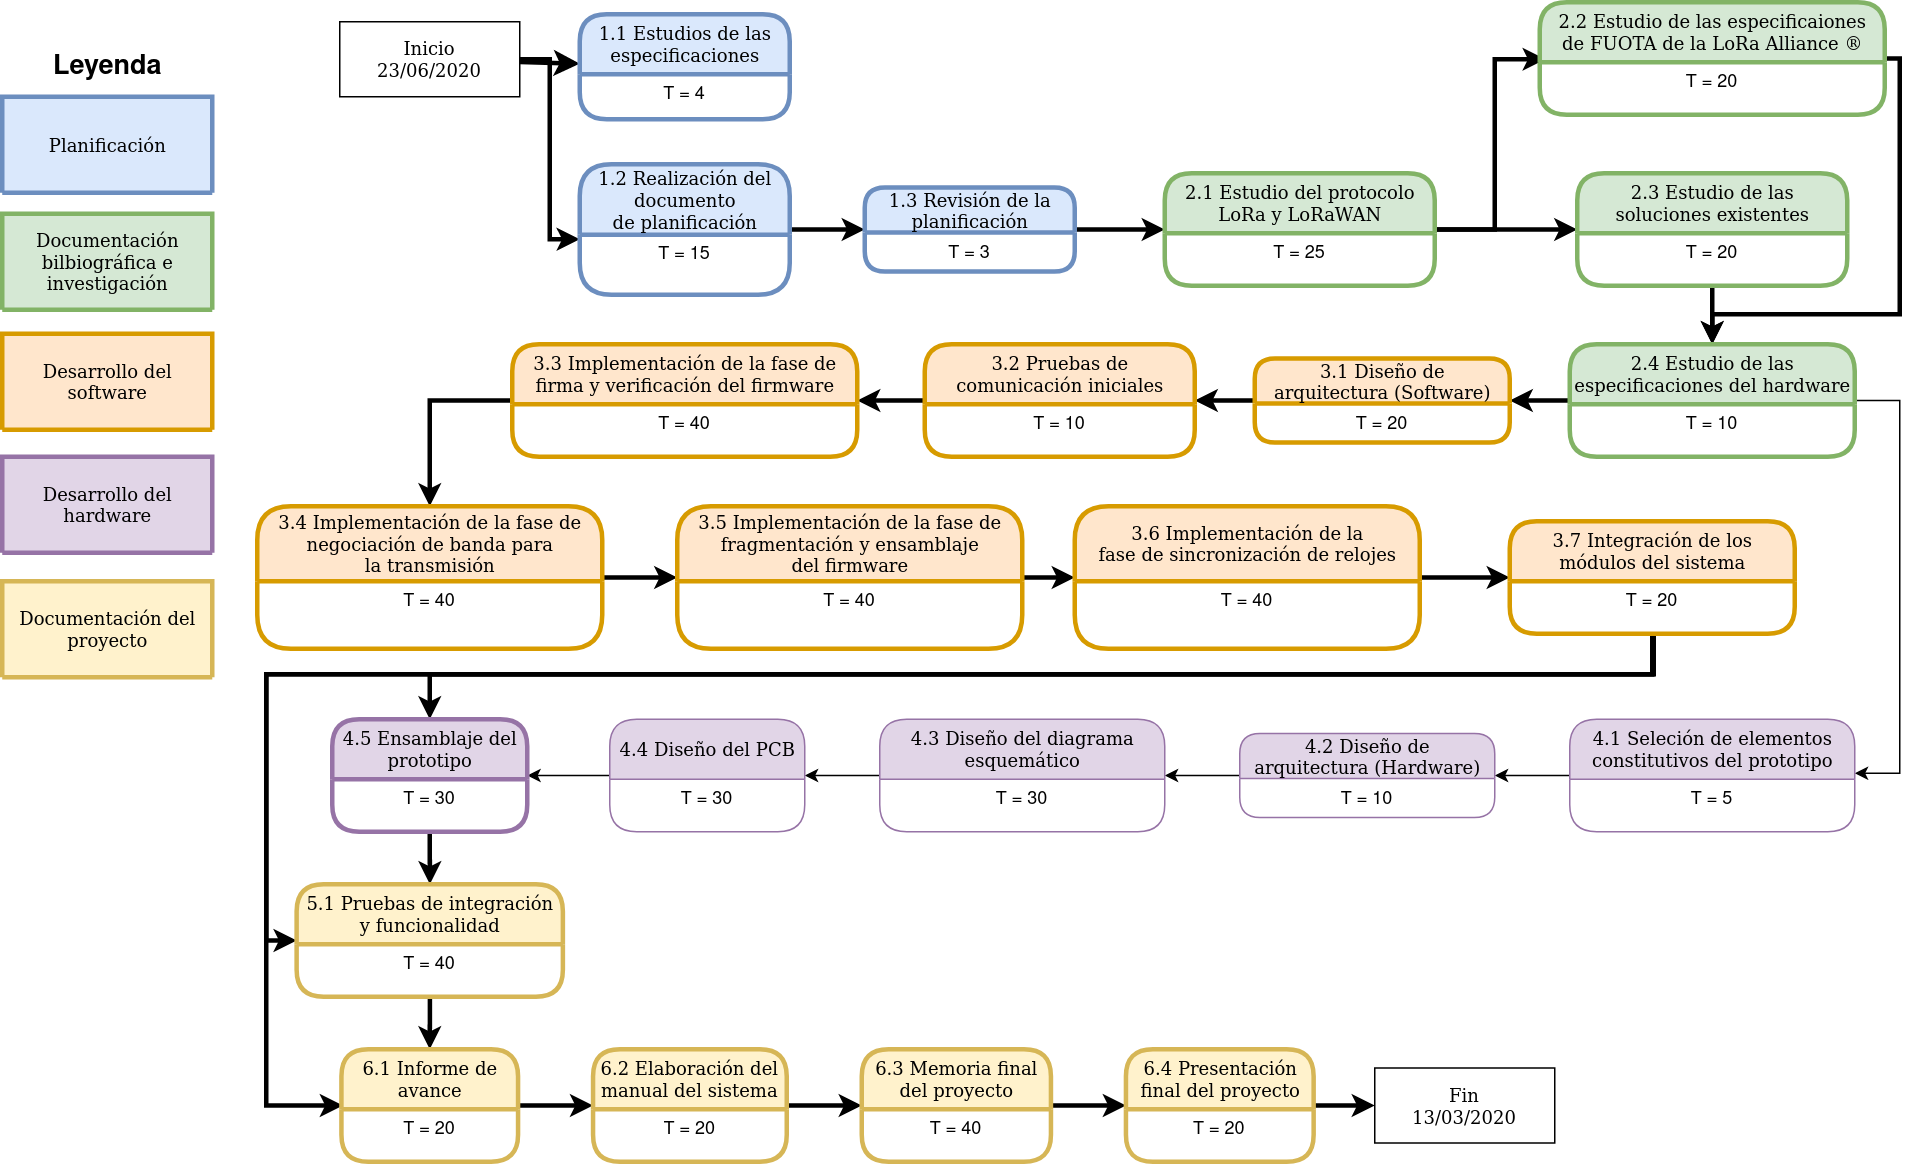
\includegraphics[width=.8\textwidth]{./Figuras/AoN.png}
\caption{Diagrama en \textit{Activity on Node}}
\label{fig:AoN}
\end{figure}

Indicar claramente en qué unidades están expresados los tiempos.
De ser necesario indicar los caminos semicríticos y analizar sus tiempos mediante un cuadro.
Es recomendable usar colores y un cuadro indicativo describiendo qué representa cada color, como se muestra en el siguiente ejemplo:



\section{8. Diagrama de Gantt}
\label{sec:gantt}

\begin{consigna}{red}
Utilizar el software Gantter for Google Drive o alguno similar para dibujar el diagrama de Gantt.

Existen muchos programas y recursos \textit{online} para hacer diagramas de gantt, entre las cuales destacamos:

\begin{itemize}
\item Planner
\item GanttProject
\item Trello + \textit{plugins}. En el siguiente link hay un tutorial oficial: \\ \url{https://blog.trello.com/es/diagrama-de-gantt-de-un-proyecto}
\item Creately, herramienta online colaborativa. \\\url{https://creately.com/diagram/example/ieb3p3ml/LaTeX}
\item Se puede hacer en latex con el paquete \textit{pgfgantt}\\ \url{http://ctan.dcc.uchile.cl/graphics/pgf/contrib/pgfgantt/pgfgantt.pdf}
\end{itemize}

Pegar acá una captura de pantalla del diagrama de Gantt, cuidando que la letra sea suficientemente grande como para ser legible. 
Si el diagrama queda demasiado ancho, se puede pegar primero la ``tabla'' del Gantt y luego pegar la parte del diagrama de barras del diagrama de Gantt.

Configurar el software para que en la parte de la tabla muestre los códigos del EDT (WBS).\\
Configurar el software para que al lado de cada barra muestre el nombre de cada tarea.\\
Revisar que la fecha de finalización coincida con lo indicado en el Acta Constitutiva.

En la figura \ref{fig:gantt}, se muestra un ejemplo de diagrama de gantt realizado con el paquete de \textit{pgfgantt}. En la plantilla pueden ver el código que lo genera y usarlo de base para construir el propio.

\begin{figure}[htbp]
\begin{center}
\begin{ganttchart}{1}{12}
  \gantttitle{2020}{12} \\
  \gantttitlelist{1,...,12}{1} \\
  \ganttgroup{Group 1}{1}{7} \\
  \ganttbar{Task 1}{1}{2} \\
  \ganttlinkedbar{Task 2}{3}{7} \ganttnewline
  \ganttmilestone{Milestone o hito}{7} \ganttnewline
  \ganttbar{Final Task}{8}{12}
  \ganttlink{elem2}{elem3}
  \ganttlink{elem3}{elem4}
\end{ganttchart}
\end{center}
\caption{Diagrama de gantt de ejemplo}
\label{fig:gantt}
\end{figure}

\end{consigna}

\section{9. Matriz de uso de recursos de materiales}
\label{sec:recursos}


\begin{table}[htpb]
\label{tab:recursos}
\centering
\begin{tabularx}{\linewidth}{@{}|c|X|X|X|X|X|@{}}
\hline
\cellcolor[HTML]{C0C0C0} & \cellcolor[HTML]{C0C0C0} & \multicolumn{4}{c|}{\cellcolor[HTML]{C0C0C0}Recursos requeridos (horas)} \\ \cline{3-6} 
\multirow{-2}{*}{\cellcolor[HTML]{C0C0C0}\begin{tabular}[c]{@{}c@{}}Código\\ WBS\end{tabular}} & \multirow{-2}{*}{\cellcolor[HTML]{C0C0C0}\begin{tabular}[c]{@{}c@{}}Nombre \\ tarea\end{tabular}} & Material 1 & Material 2 & Material 3 & Material 4 \\ \hline
 &  &  &  &  &  \\ \hline
 &  &  &  &  &  \\ \hline
 &  &  &  &  &  \\ \hline
 &  &  &  &  &  \\ \hline
\end{tabularx}%
\end{table}


\section{10. Presupuesto detallado del proyecto}
\label{sec:presupuesto}

\begin{consigna}{red}
Si el proyecto es complejo entonces separarlo en partes:
\begin{itemize}
\item Un total global, indicando el subtotal acumulado por cada una de las áreas.
\item El desglose detallado del subtotal de cada una de las áreas.
\end{itemize}

IMPORTANTE: No olvidarse de considerar los COSTOS INDIRECTOS.

\end{consigna}

\begin{table}[htpb]
\centering
\begin{tabularx}{\linewidth}{@{}|X|c|r|r|@{}}
\hline
\rowcolor[HTML]{C0C0C0} 
\multicolumn{4}{|c|}{\cellcolor[HTML]{C0C0C0}COSTOS DIRECTOS} \\ \hline
\rowcolor[HTML]{C0C0C0} 
Descripción &
  \multicolumn{1}{c|}{\cellcolor[HTML]{C0C0C0}Cantidad} &
  \multicolumn{1}{c|}{\cellcolor[HTML]{C0C0C0}Valor unitario} &
  \multicolumn{1}{c|}{\cellcolor[HTML]{C0C0C0}Valor total} \\ \hline
 &
  \multicolumn{1}{c|}{} &
  \multicolumn{1}{c|}{} &
  \multicolumn{1}{c|}{} \\ \hline
 &
  \multicolumn{1}{c|}{} &
  \multicolumn{1}{c|}{} &
  \multicolumn{1}{c|}{} \\ \hline
\multicolumn{1}{|l|}{} &
   &
   &
   \\ \hline
\multicolumn{1}{|l|}{} &
   &
   &
   \\ \hline
\multicolumn{3}{|c|}{SUBTOTAL} &
  \multicolumn{1}{c|}{} \\ \hline
\rowcolor[HTML]{C0C0C0} 
\multicolumn{4}{|c|}{\cellcolor[HTML]{C0C0C0}COSTOS INDIRECTOS} \\ \hline
\rowcolor[HTML]{C0C0C0} 
Descripción &
  \multicolumn{1}{c|}{\cellcolor[HTML]{C0C0C0}Cantidad} &
  \multicolumn{1}{c|}{\cellcolor[HTML]{C0C0C0}Valor unitario} &
  \multicolumn{1}{c|}{\cellcolor[HTML]{C0C0C0}Valor total} \\ \hline
\multicolumn{1}{|l|}{} &
   &
   &
   \\ \hline
\multicolumn{1}{|l|}{} &
   &
   &
   \\ \hline
\multicolumn{1}{|l|}{} &
   &
   &
   \\ \hline
\multicolumn{3}{|c|}{SUBTOTAL} &
  \multicolumn{1}{c|}{} \\ \hline
\rowcolor[HTML]{C0C0C0}
\multicolumn{3}{|c|}{TOTAL} &
   \\ \hline
\end{tabularx}%
\end{table}


\section{11. Matriz de asignación de responsabilidades}
\label{sec:responsabilidades}
\begin{consigna}{red}
Establecer la matriz de asignación de responsabilidades y el manejo de la autoridad completando la siguiente tabla:

\begin{table}[htpb]
\centering
\resizebox{\textwidth}{!}{%
\begin{tabular}{|c|c|c|c|c|c|}
\hline
\rowcolor[HTML]{C0C0C0} 
\cellcolor[HTML]{C0C0C0} &
  \cellcolor[HTML]{C0C0C0} &
  \multicolumn{4}{c|}{\cellcolor[HTML]{C0C0C0}Listar todos los nombres y roles del proyecto} \\ \cline{3-6} 
\rowcolor[HTML]{C0C0C0} 
\cellcolor[HTML]{C0C0C0} &
  \cellcolor[HTML]{C0C0C0} &
  Responsable &
  Orientador &
  Equipo &
  Cliente \\ \cline{3-6} 
\rowcolor[HTML]{C0C0C0} 
\multirow{-3}{*}{\cellcolor[HTML]{C0C0C0}\begin{tabular}[c]{@{}c@{}}Código\\ WBS\end{tabular}} &
  \multirow{-3}{*}{\cellcolor[HTML]{C0C0C0}Nombre de la tarea} &
  \authorname &
  \supname &
  Nombre de alguien &
  \clientename \\ \hline
 &  &  &  &  &  \\ \hline
 &  &  &  &  &  \\ \hline
 &  &  &  &  &  \\ \hline
\end{tabular}%
}
\end{table}

{\footnotesize
Referencias:
\begin{itemize}
	\item P = Responsabilidad Primaria
	\item S = Responsabilidad Secundaria
	\item A = Aprobación
	\item I = Informado
	\item C = Consultado
\end{itemize}
} %footnotesize

Una de las columnas debe ser para el Director, ya que se supone que participará en el proyecto.
A su vez se debe cuidar que no queden muchas tareas seguidas sin ``A'' o ``I''.

Importante: es redundante poner ``I/A'' o ``I/C'', porque para aprobarlo o responder consultas primero la persona debe ser informada.

\end{consigna}

\section{12. Gestión de riesgos}
\label{sec:riesgos}

\begin{consigna}{red}
a) Identificación de los riesgos (al menos cinco) y estimación de sus consecuencias:
 
Riesgo 1: detallar el riesgo (riesgo es algo que si ocurre altera los planes previstos)
\begin{itemize}
\item Severidad (S): mientras más severo, más alto es el número (usar números del 1 al 10).\\
Justificar el motivo por el cual se asigna determinado número de severidad (S).
\item Probabilidad de ocurrencia (O): mientras más probable, más alto es el número (usar del 1 al 10).\\
Justificar el motivo por el cual se asigna determinado número de (O). 
\end{itemize}   

Riesgo 2:
\begin{itemize}
\item Severidad (S): 
\item Ocurrencia (O):
\end{itemize}

Riesgo 3:
\begin{itemize}
\item Severidad (S): 
\item Ocurrencia (O):
\end{itemize}


b) Tabla de gestión de riesgos:      (El RPN se calcula como RPN=SxO)

\begin{table}[htpb]
\centering
\begin{tabularx}{\linewidth}{@{}|X|c|c|c|c|c|c|@{}}
\hline
\rowcolor[HTML]{C0C0C0} 
Riesgo & S & O & RPN & S* & O* & RPN* \\ \hline
       &   &   &     &    &    &      \\ \hline
       &   &   &     &    &    &      \\ \hline
       &   &   &     &    &    &      \\ \hline
       &   &   &     &    &    &      \\ \hline
       &   &   &     &    &    &      \\ \hline
\end{tabularx}%
\end{table}

Criterio adoptado: 
Se tomarán medidas de mitigación en los riesgos cuyos números de RPN sean mayores a ....

Nota: los valores marcados con (*) en la tabla corresponden luego de haber aplicado la mitigación.

c) Plan de mitigación de los riesgos que originalmente excedían el RPN máximo establecido:
 
Riesgo 1: Plan de mitigación (si por el RPN fuera necesario elaborar un plan de mitigación).
  Nueva asignación de S y O, con su respectiva justificación:
  - Severidad (S): mientras más severo, más alto es el número (usar números del 1 al 10).
          Justificar el motivo por el cual se asigna determinado número de severidad (S).
  - Probabilidad de ocurrencia (O): mientras más probable, más alto es el número (usar del 1 al 10).
          Justificar el motivo por el cual se asigna determinado número de (O).

Riesgo 2: Plan de mitigación (si por el RPN fuera necesario elaborar un plan de mitigación).
 
Riesgo 3: Plan de mitigación (si por el RPN fuera necesario elaborar un plan de mitigación)

\end{consigna}


\section{13. Gestión de la calidad}
\label{sec:calidad}

\begin{consigna}{red}
Para cada uno de los requerimientos del proyecto indique:
\begin{itemize} 
\item Req \#1: Copiar acá el requerimiento.

Verificación y validación:

\begin{itemize}
\item Verificación para confirmar si se cumplió con lo requerido antes de mostrar el sistema al cliente:\\
Detallar 
\item Validación con el cliente para confirmar que está de acuerdo en que se cumplió con lo requerido:\\
Detallar  
\end{itemize}

\end{itemize}

Tener en cuenta que en este contexto se pueden mencionar simulaciones, cálculos, revisión de hojas de datos, consulta con expertos, etc.

\end{consigna}

\section{14. Comunicación del proyecto}
\label{sec:comunicaciones}

\begin{consigna}{red}
El plan de comunicación del proyecto es el siguiente:
\end{consigna}

% Please add the following required packages to your document preamble:
% \usepackage{graphicx}
% \usepackage[table,xcdraw]{xcolor}
% If you use beamer only pass "xcolor=table" option, i.e. \documentclass[xcolor=table]{beamer}
\begin{table}[htpb]
\centering
\resizebox{\textwidth}{!}{%
\begin{tabular}{|c|c|c|c|c|c|}
\hline
\rowcolor[HTML]{C0C0C0} 
\multicolumn{6}{|c|}{\cellcolor[HTML]{C0C0C0}PLAN DE COMUNICACIÓN DEL PROYECTO}           \\ \hline
\rowcolor[HTML]{C0C0C0} 
¿Qué comunicar? & Audiencia & Propósito & Frecuencia & Método de comunicac. & Responsable \\ \hline
                &           &           &            &                      &             \\ \hline
                &           &           &            &                      &             \\ \hline
                &           &           &            &                      &             \\ \hline
                &           &           &            &                      &             \\ \hline
                &           &           &            &                      &             \\ \hline
\end{tabular}%
}
\end{table}

\section{15. Gestión de Compras}
\label{sec:compras}

\begin{consigna}{red}
En caso de tener que comprar elementos o contratar servicios:
a) Explique con qué criterios elegiría a un proveedor.
b) Redacte el Statement of Work correspondiente.
\end{consigna}

\section{16. Seguimiento y control}
\label{sec:seguimiento}

\begin{consigna}{red}
Para cada tarea del proyecto establecer la frecuencia y los indicadores con los se seguirá su avance y quién será el responsable de hacer dicho seguimiento y a quién debe comunicarse la situación (en concordancia con el Plan de Comunicación del proyecto).

El indicador de avance tiene que ser algo medible, mejor incluso si se puede medir en \% de avance. Por ejemplo,se pueden indicar en esta columna cosas como ``cantidad de conexiones ruteadeas'' o ``cantidad de funciones implementadas'', pero no algo genérico y ambiguo como ``\%'', porque el lector no sabe porcentaje de qué cosa.

\end{consigna}

\begin{table}[!htpb]
\centering
\begin{tabularx}{\linewidth}{@{}|X|X|X|X|X|X|@{}}
\hline
\rowcolor[HTML]{C0C0C0} 
\multicolumn{6}{|c|}{\cellcolor[HTML]{C0C0C0}SEGUIMIENTO DE AVANCE}                                                                       \\ \hline
\rowcolor[HTML]{C0C0C0} 
Tarea del WBS & Indicador de avance & Frecuencia de reporte & Resp. de seguimiento & Persona a ser informada & Método de comunic. \\ \hline
 &  &  &  &  &  \\ \hline
 &  &  &  &  &  \\ \hline
 &  &  &  &  &  \\ \hline
 &  &  &  &  &  \\ \hline
 &  &  &  &  &  \\ \hline
\end{tabularx}%
%}
\end{table}

\section{17. Procesos de cierre}    
\label{sec:cierre}

\begin{consigna}{red}
Establecer las pautas de trabajo para realizar una reunión final de evaluación del proyecto, tal que contemple las siguientes actividades:

\begin{itemize}
\item Pautas de trabajo que se seguirán para analizar si se respetó el Plan de Proyecto original:
 - Indicar quién se ocupará de hacer esto y cuál será el procedimiento a aplicar. 
\item Identificación de las técnicas y procedimientos útiles e inútiles que se utilizaron, y los problemas que surgieron y cómo se solucionaron:
 - Indicar quién se ocupará de hacer esto y cuál será el procedimiento para dejar registro.
\item Indicar quién organizará el acto de agradecimiento a todos los interesados, y en especial al equipo de trabajo y colaboradores:
  - Indicar esto y quién financiará los gastos correspondientes.
\end{itemize}

\end{consigna}

\end{document}
